\chapter{Network Basics}\label{ch:06-net-use}

\section{Bandwidth and Latency}

When using a network, there are two things we care about most: speed an reliability.
Speed is measured by two metrics, bandwidth and latency, which we discuss here.
Reliability depends, too a large degree, on topology, which we will discuss later.

\df{Bandwidth} is the amount of information transmitted per unit time.
\df{Latency} is the amount of time it takes for information to travel
  from source to target.
As an example,
  let us estimate the bandwidth and the latency
  of a network link between London and Paris,
  which is implemented by USB-carrying pigeons.
For this example,
  we assume an infinite supply of well-trained pigeons,
  and we neglect the small number of pigeons that are shot in flight.
What is the bandwidth?
Somebody needs to attach USB drives to pigeons.
We need to estimate how much time this takes,
  and we also need to estimate how much information fits in an USB drive.
Somebody who attaches USB drives to pigeons for a living
  can probably do a good job in 1~minute.
As for the size of the USB drive,
  let us err on the cheap side: we will be using 2~GiB drives.
So, what's the bandwidth?
\[
\frac{2\,{\rm GiB}}{1\.{\rm minute}}
  = \frac{2^{34}\,{\rm b}}{60\,{\rm s}}
  > 280\times 10^6 {\rm b}/{\rm s}
\]
A 280~Mbps Internet connection is rather fast!
So, why are not we all using pigeon-based Internet?
One reason is clear: well trained pigeons are hard to come by;
  in other words,
  our assumption that we have an infinite supply of such pigeons is unrealistic.
But, there's another reason: latency is pretty bad.
Let's see: how long does it take a pigeon to travel from London to Paris?
The distance (as a pigeon would fly) is about 300~km.
Good pigeons attain average speeds of 125~km/h.
Thus, latency is
\[
\frac{300\,{\rm km}}{125\,{\rm km}/{\rm h}}
  = 2.4\,{\rm h} = 8640\,{\rm s}
\]
With a latency on the order of tens of thousands of seconds,
  pigeon-based Internet makes a poor choice for certain applications
  that require interactivity, such as video-chats.

Now, let us compare these numbers with those of the real Internet,
  as seen on University of Kent's campus.
\begin{verbatim}
rg@rg-2016:temp$ curl -o dblp.xml.gz http://dblp.uni-trier.de/xml/dblp.xml.gz
  % Total    % Received % Xferd  Average Speed   Time    Time     Time  Current
                                 Dload  Upload   Total   Spent    Left  Speed
100  363M  100  363M    0     0  5057k      0  0:01:13  0:01:13 --:--:-- 5050k
\end{verbatim}
So, the bandwidth is
\[
  5057\,{\rm KB}/{\rm s} = 5057\times1024\times8\,{\rm b}/{\rm s}
    < 42\times10^6\,{\rm b}/{\rm s}
\]
That's $6.7$~times worse than using pigeons!
What about latency?
\begin{verbatim}
rg@rg-2016:temp$ ping -c 3 dblp.uni-trier.de
PING dblp.uni-trier.de (136.199.55.186) 56(84) bytes of data.
64 bytes from dblp.uni-trier.de (136.199.55.186): icmp_seq=1 ttl=44 time=16.8 ms
64 bytes from dblp.uni-trier.de (136.199.55.186): icmp_seq=2 ttl=44 time=17.8 ms
64 bytes from dblp.uni-trier.de (136.199.55.186): icmp_seq=3 ttl=44 time=17.6 ms

--- dblp.uni-trier.de ping statistics ---
3 packets transmitted, 3 received, 0% packet loss, time 2003ms
rtt min/avg/max/mdev = 16.878/17.452/17.815/0.410 ms
\end{verbatim}
The latency is $<17.5/2\,{\rm ms}<0.01\,{\rm s}$,
  which is \emph{much} smaller than that of the pigeons.
(True, I'm not quite sure where the DBLP server is,
  but I suspect it's not closer than Paris.)
The division by~$2$ is there because \.{ping} reports
  the rtt ({\bf r}ound {\bf t}rip {\bf t}ime),
  which is twice the latency.

You may complain that pigeons make a poor, artificial example of data carriers.
If you think so,
  then imagine that instead of pigeons one uses trucks filled with hard drives.
That is definitely \emph{not} an artificial example:
  Google `AWS Snowmobile'!


\section{Topology}

Networks are made of many interconnected computers.
The most important property of a network is its \df{topology}:
  which computers can communicate directly.
The following figure shows two simple topologies: a ring and a star.
\begin{center}
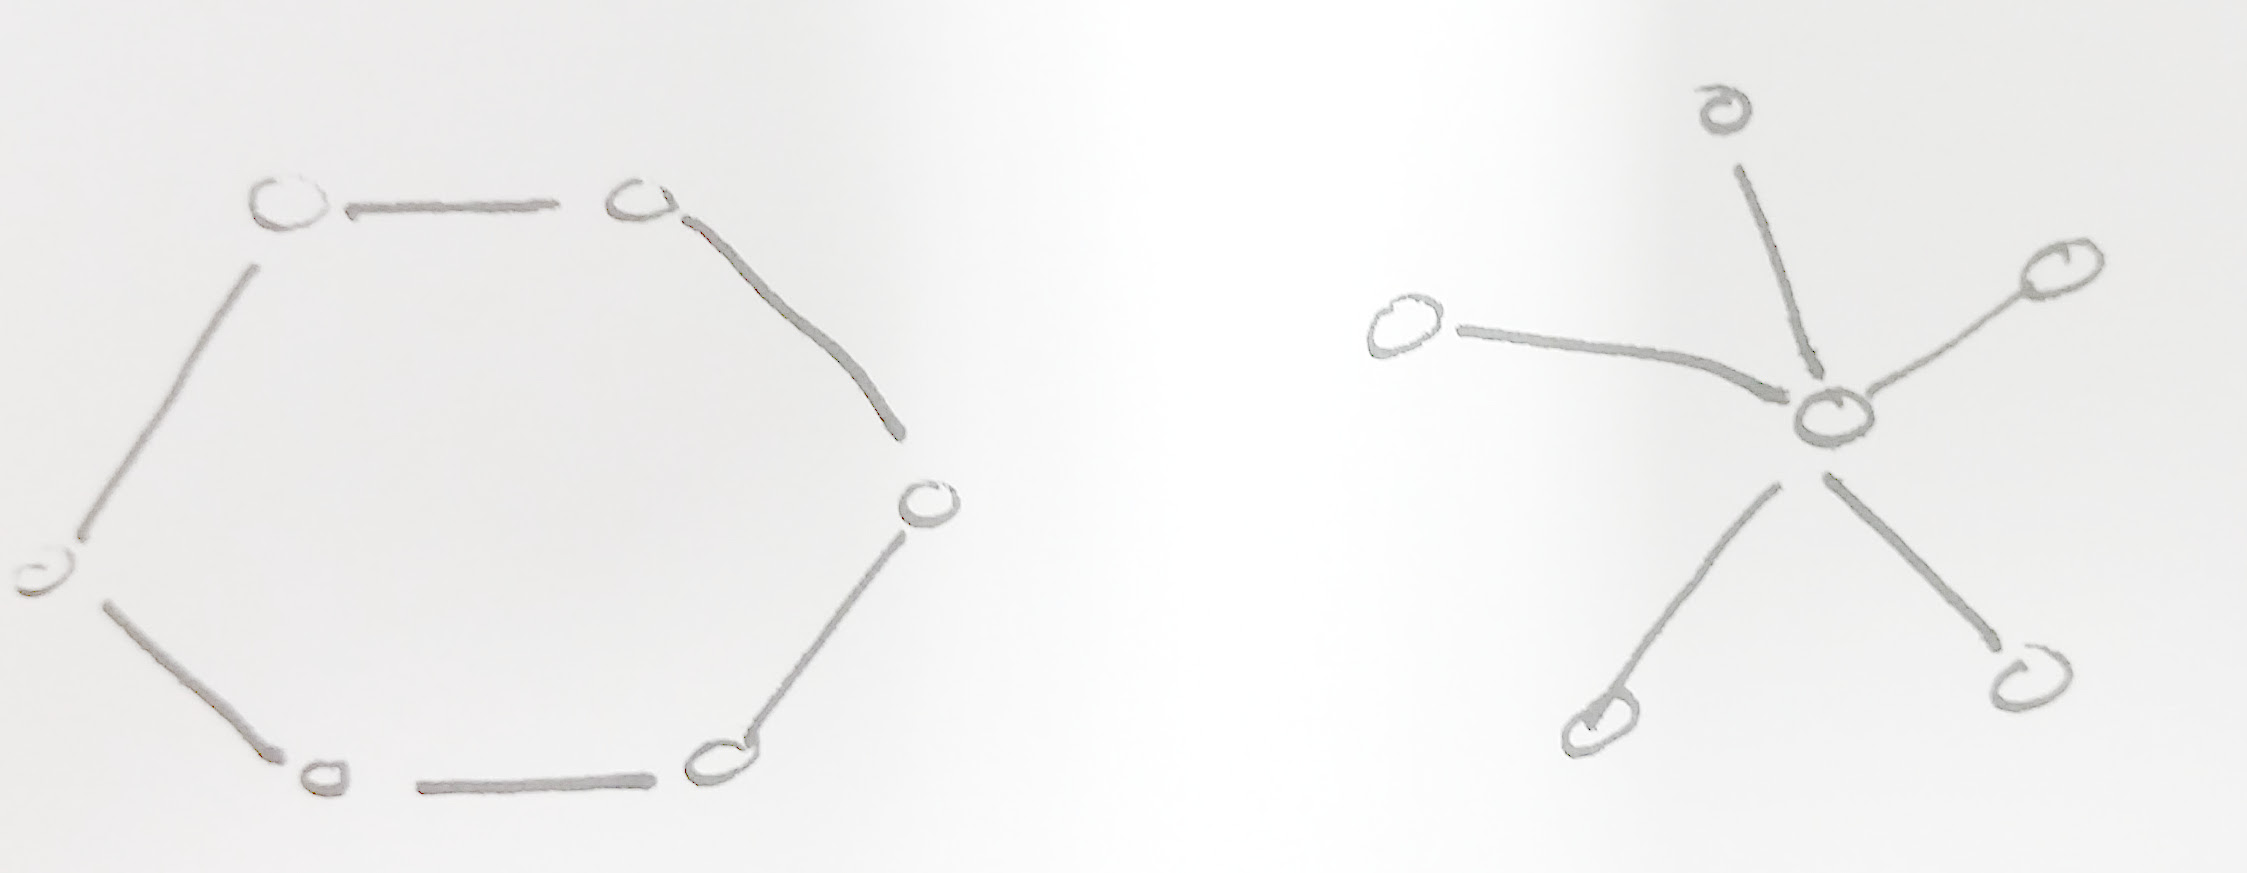
\includegraphics[width=0.6\textwidth]{ring-star.jpg}
\end{center}
\todo{tikz drawing}
In both cases, we have 6~network nodes (the circles).
In the ring on the left, there are 6~network links;
in the star on the right, there are 5~network links.
The \df{distance} between two nodes is the minimum number of links
  that need to be used to communicate.
In the ring on the left,
  the distance can be 1, 2, or 3, depending on which pair of nodes we talk about;
in the star on the right,
  the distance can be 1 or 2, depending on whether the center node is involved.
The \df{diameter} of a network is the largest distance between a pair of its nodes.
The ring in our example has diameter~3;
the star has diameter 2.
A set of links is said to be a \df{cut} of the network,
  if the failure of these links would lead to partitioning the network
    in $\ge2$ components.
The \df{minimum cut} of a network is the smallest size of a cut.
The ring has minimum cut~2;
  the star has minimum cut~1.

All these measures are rather abstract.
That makes them applicable in a wide array of situations.
And, such measures are surprisingly useful.
For example,
  the minimum cut gives a simple way to asses the reliability of a network.

\section{Packets and Layers}

Computer networks resemble less the telephone system and more the mail system.
To send mail, you put your writing in an envelope.
On the envelope, there is some more writing,
  which is not what you want to communicate
  but helps the envelope arrive at its destination.
The writing on the envelope includes, of course,
  the address of the destination.
In computer networks, the story is similar.
The information you want to transmit is split into discrete units called packets.
Each packet has a part to be delivered (the \df{payload})
  and a part that helps in making the delivery (the \df{headers}).
The payload is like the letter you mail;
  the headers are like the envelope in which you put your letter.

But, computer networks are more complicated than the mail system,
  because they put envelopes in envelopes in envelopes \dots
The following picture illustrates how information is sent in the Internet.
\begin{center}
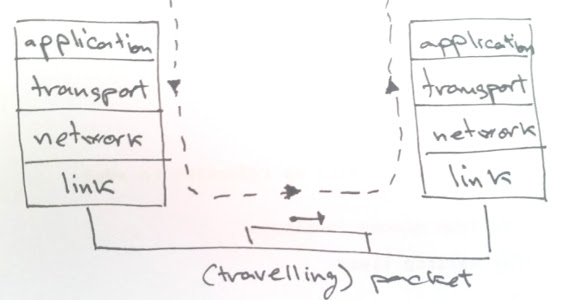
\includegraphics[width=.6\textwidth]{network-layers.jpg}
\end{center}
\todo{tikz}
Let us look see what happens
  when the user on the left wants to send a message to the user on the right.
\begin{enumerate}
\item
  The user on the left passes the message to its application layer.
\item
  The application layer adds its headers,
    and then passes the packet down to the transport layer.
\item
  The transport layer adds its headers,
    and then passes the packet down to the network layer.
\item
  The network layer adds its headers,
    and then passes the packet down to the link layer.
\item
  The link layer adds its headers,
    and then physically transmits the packet to another network node.
\item \dots
\item
  The link layer of the user on the right strips the link-layer headers,
    and then passes the packet up to the network layer.
\item
  The network layer strips the network-layer headers,
    and then passes the packet up to the transport layer.
\item
  The transport layer strips the transport-layer headers,
    and then passes the packet up to the application layer.
\item
  \emph{Finally}, the application layer strips the application-layer headers,
    and passes the message to the user on the right.
\end{enumerate}
In short, the information flows as the dashed line shows.

Why are there so many layers?
Each of them has different responsibilities.
\todo{Define layer/protocol.}

Examples protocols within the link layer are WLAN and Ethernet.
The main responsibility of the link layer is to transmit information physically.
Two computers that are linked will exchange some packets that carry user messages,
  but also some packets that are necessary for coordinating how information
    is transmitted.
For example, a wireless access point regularly transmits a \emph{beacon},
  to advertise its presence.

The most known protocol within the network layer is IP (Internet Protocol).
The main responsibility of the network layer is to route packets.
This job is quite similar to sorting mail:
  you look at the address on the envelope,
    and you decide where to send the envelope next.
To carry out this task, network protocols must have a notion of \df{address}.
An \df{IPv4 address} is 32~bit number;
  an \df{IPv6 address} is a 128~bit number.
Each node in the network maintains routing tables,
  which contain entries of the following form:
\begin{center}
if the destination address starts with $\it foo$,\\
  then I'll forward the packet to my neighbour $\it bar$
\end{center}
Somebody needs to create these routing tables in the first place.
This can be done in different ways.
One option is to use a fully automatic routing protocol,
  such as OSPF or IS-IS\null.
These protocols do not scale to the whole of Internet, though.
Another option is to use a semi-automatic routing protocol like BGP\null.
Semi-automatic means that humans provide some high-level rules,
  and the protocol needs to work out the routing table entries.
OSPF and IS-IS are used for the networks
  of companies that own a big part of the Internet;
  that is, inside a \emph{domain}.
BGP is used for inter-domain routing in the Internet.

The network layer does not guarantee that packets reach their destination.

Examples of protocols within the transport layer are
  UDP ({\bf u}ser {\sf d}atagram {\bf p}rotocol) and
  TCP ({\bf t}ransmission {\bf c}ontrol {\bf p}rotocol).
UDP does not really do much more than what IP does,
  except it introduces a notion of a \emph{port} that refines an address.
(This is like saying that you write on the envelope not only the house name,
  but also the name of the person who should open the letter.)
TCP, on the other hand, ensures that
  (1)~bytes reach their destination,
  (2)~in the order they were sent.
Both these guarantees are \emph{not} available with UDP (or IP).
TCP achieves this by using sequence numbers and retransmissions.
Because of these (especially because of retransmissions),
  TCP has poor latency, compared to UDP.

The most known protocol within the application layer is HTTP\null.
Application protocols are not implemented in the operating system.
Usually, they are implemented in software libraries.
For example,
  in C++ one could use the library \.{libcurl};
  in Java one would use \.{java.net} from the standard library;
  in Python one would use \.{urllib} from the standard library,
    or the library \.{requests};
  and so on.

\smallskip

We already saw an example of inaccuracy in the previous picture:
  the packet is not simply passed down the layer stack,
    transmitted, and then passed up the layer stack,
    because sometimes retransmissions are necessary.
Another inaccuracy in the picture is that there are no intermediate nodes.
In general, the two computers that communicate are rarely neighbours.
Intermediate nodes often have mini-stacks,
  which include only the link and network layers.
Such intermediate nodes are called \df{routers}.

One may connect together several networks, to build an inter-network.
(The biggest inter-network was baptized Internet.)
\begin{center}
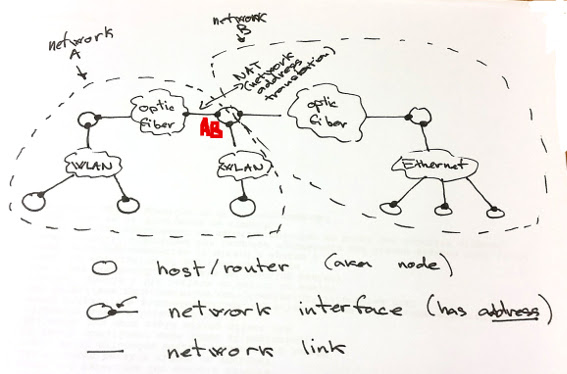
\includegraphics[width=.9\textwidth]{internetwork.jpg}
\end{center}
\todo{tikz}
In the picture we see that computers can have several network interfaces.
Computers do not really have network addresses: their network interfaces do.
A \df{network} is a domain of visibility for network addresses;
  or, otherwise put,
    it is a set of network interfaces that must have \emph{unique}
      network addresses.
How do computers in different networks communicate?
The basic idea is that one computer is connected to both networks,
  through two network interfaces.
If a computer in network~A wants to communicate with a computer in network~B,
  then it will use the address (in network~A) of the computer~AB.
It also needs to indicate somehow what is the intended destination in network~B\null.
One way to do so, is to use a particular port number.
Then computer~AB has a table with entries of the form:
\begin{center}
  if a packet comes on port $\it foo$ in network~A,\\
    then I should send it along to network~B with destination address~$\it bar$
\end{center}
The mapping ${\it foo}\mapsto{\it bar}$ is a matter of configuration,
  by sysadmins.
Applying such rules to forward packets from one network to another
  is called \df{NAT} ({\bf n}etwork {\bf a}ddress {\bf t}ranslation).

\smallskip

We saw that the application layer is usually implemented outside the operating system.
The transport and network layers are usually implemented in the operating system.
The link layer is partly implemented in the operating system,
  and partly in hardware components such as wireless network cards.

\section{Socket Programming}

The interface offered by the operating system uses sockets.
In other words,
  the application layer discusses with the transport layer through sockets.

A connected socket is similar to an open file.
A connected socket is identified by an integer,
  just like an open file is identified by a file descriptor which is an integer.
We can use a connected socket in most places where we can use a file descriptor.
In particular, we can use the functions \.{read}, \.{write}, and \.{select}.

To obtain a connected socket we must establish a network connection.
Establishing a network connection is asymmetric:
  the client initiates the connection,
  while the server waits for connections.

Here is what the client must do:
\begin{ccode}
int s = socket(AF_INET, SOCK_STREAM, 0);
connect(s, (struct sockaddr *) &address, sizeof address);
\end{ccode}
Line~1 creates a socket; line~2 connects to a server.
We will see later how \.{address} is set.
After line~2, the client can use the functions \.{read} and \.{write}
  as if \.{s} were a file descriptor.

Here is what the server must do:
\begin{ccode}
int listening_socket = socket(AF_INET, SOCK_STREAM, 0);
bind(listening_socket, (struct sockaddr *) &address, sizeof address);
listen(listening_socket, connection_queue_size);
int connected_socket = accept(listening_socket, NULL, NULL);
\end{ccode}
Line~1 creates a socket;
  line~2 binds the socket to a local address;
  line~3 prepares this socket to accept connections;
  line~4 accepts a connection.
In line~1, we choose which type of socket to use.
In line~2, we choose where to wait for connections:
  a computer may have multiple network interfaces,
  and even single network interfaces have several ports.
In line~3, we choose how many clients can queue waiting for a connection;
  if more clients try to connect, they will be summarily refused.
In line~4, we obtain a connected socket,
  which is \emph{different} from the listening socket:
  we use \.{connected\_socket} as if it were a file, to communicate with the client;
  we use \.{listening\_socket} to \.{accept} further connections.

At this point, both the client and the server can communicate
  using the functions \.{read} and \.{write},
  as if they would be interacting with an open file.
See the accompanying \.{miniclient.c} and \.{miniserver.c}.


\section{Exercises}

\begin{enumerate}
\item
  $\blacktriangleright$
  What is a \emph{socket}?
\item
  Look at Java's implementation of
    \.{java.net.Socket} and \.{java.net.DatagramSocket}.
\item
  Look at `\.{man getaddrinfo}'.
\end{enumerate}

% vim:spell:spelllang=en_gb:
